\setcounter{figure}{0}
\renewcommand{\thefigure}{5-\arabic{figure}}

\section[第五章\q 雕虫小技]{第五章\\ 雕虫小技}

\subsection{股市层次理论}

{\kaishu
波浪理论的真谛不在于精确地数浪，而在于其蕴含的宝贵思想。

\hfill ——金融帝国
}

股市上牛市与熊市交替出现，从而形成了一种牛熊循环。那么这种循环从市场内部来看，是否有某种规律可言呢？如果以个股间涨跌的分化与集中程度来划分，那么确实能够找出市场规律的一些蛛丝马迹。这套理论起源于早期对波浪理论的研究，希望找出股市在不同波浪中的市场内部特征。那时我发现，股市的三浪上扬通常是全部个股的一致性上涨；而五浪上扬通常表现为不同类型股票的分化上涨；A浪下跌通常是全部个股的一致性下跌；而C浪下跌通常表现为不同类型股票的分化下跌。

后来我发现，这套理论虽然能够很好地解释市场，但有时又并非与波浪理论的划分完全一致。甚至波浪理论在复杂的市场面前，虽然从宏观上来说是完美的，但从微观上来看通常又并非完全吻合。有意思的是：即使不考虑波浪理论，这套理论也是成立的，甚至能够对市场进行更好的分析。这样一来，我就跳出波浪理论的束缚，建立了一种更宏观的市场划分方法。

市场的循环可以划分为：绝对牛市——换档——相对牛市——绝对熊市——换档——相对熊市。所谓“绝对”就是指全部股票一致性地集中波动；所谓“相对”就是不同股票不同步地分化波动。为了方便下面的验证，我们把市场上的全部股票划分为三大类。第一类，低价大盘股。这类股票是市场上的巨无霸，具有庞大的股本，同时价位通常较低。第二类，绩优股。这类股票有不错的业绩支撑。第三类，绩差股（题材股）。这类股票业绩比较差，甚至亏损。

1996年的绝对牛市：无论是以上海石化为首的低价大盘股，还是以长虹、深科技为首的绩优股，或者是北京天桥之类的绩差股，都走出了大幅上涨的行情。即使垃圾股启动较晚，但在行情的中后期也走出了成倍的升幅。由此可见，绝对牛市中买入弱势股等待补涨，也并非不可取。

1996年底的换档：《人民日报》社论将过热的股市快速打压下来。虽然绩差股大幅跳水，将曾经的上涨吞没了绝大部分，但长虹、发展、深科技等绩优股拒绝调整而表现得非常抗跌。

1997年上半年的相对牛市：虽然大盘在绩优股的带领下走出笔直的上涨行情，但是低价大盘股已经无法创出1996年底的高点，而绩差股也都在1996年高点的不远处停止了上涨的脚步。

1997年下半年的绝对熊市：无论是绩优股、绩差股，还是低价大盘股都走出了下跌行情。

1998年上半年的换档：被市场唾弃的绩差股，不可思议地开始不断大幅度的飙升；而老牌绩优股和低价大盘股基本上没任何起色。

1998年下半年至1999年上半年的相对熊市：虽然老牌绩优股继续大幅下挫，直到5·19行情的起点时才最终止跌；但众多绩差股已经在历史高位拒绝调整（北京天桥等），甚至还在继续创出新高（阿城钢铁）；低价大盘股也在1998年8月的1043点见底，开始了横向整理。

1999年下半年的绝对牛市：无论是低价大盘股、绩差股，还是老牌绩优股都走出了大幅上扬的行情。其中长虹、发展也从最低点快速上涨了一倍以上；而上海石化等低价大盘股也在巨大成交量的推动下大幅飙升；绩差股更是当仁不让继续大幅上涨。

1999年下半年的换档：虽然老牌绩优股快速下跌；低价大盘股也进入调整期；但绩差股拒绝调整反而继续上涨。虽然大盘下跌了五个月，当大盘见底时，亿安科技、海虹控股、北京天桥等众多绩差股早已创出历史新高。

2000年至2001年上半年的相对牛市：垃圾股创造了不可思议的辉煌，当然那时部分垃圾股的本质虽然还是垃圾，但已经披上科技股的外衣。而老牌绩优股根本就在历史低位丝毫不动，即使真正的绩优股也没有什么起色。低价大盘股走出了小幅度的缓慢上涨，当然马钢当年表现不错，后来钢铁、水泥行业的股票也有所表现。那是一个赚钱并不容易的时期。

2001年下半年的绝对熊市：那是一个是股票就会大幅下跌的时段，无论大盘还是小盘，也无论绩优还是绩差都摆脱不了下跌的命运。垃圾股暴炒后泡沫般地破灭；老牌绩优股虽然牛市没有怎么上涨，但跌起来却并不逊色。

2002年至2004年上半年的换档：虽然更多没有业绩支撑的绩差股还在不断下跌，但这两年间汽车股首先创出2001年的新高；然后是核心资产类的中国石化、宝钢股份等，命名为“五朵金花”的低价大盘股也创出2001年的新高。

2004年下半年至2005年的相对熊市：虽然那时大盘仍旧笼罩在熊市的恐慌气氛下，大量没有业绩支撑的股票跌得惨不忍睹。但是基金重仓股却在不断走强，其中贵州茅台、大商股份、小商品城等一系列股票早已创出2001年的高点且不断攀升，当时市场称其为基金“抱团取暖”业绩优良的蓝筹股。而中国石化、宝钢股份等低价大盘股，也没有创出2003年的新低。

2006年至2007年上半年的绝对牛市：这是一个只要持股就能获利的时段。与2001年正好对称，只要是股票就能上涨。这时股民的获利能力，基本上与持股能力成正比。

2007年下半年“换档”：虽然“大幅提高印花税”的利空是否能够演化为换档行情还有待观察，但三线绩差股夺路而逃的景象与高价绩优股逆势不跌的场面形成了鲜明的对比。天文学家说，太阳的活动周期能够形成10.5年的循环，那么太阳活动周期是否能够影响人类的活动行为呢？是否现在我们又在经历1996年底上演的一幕呢？（本书的测试版写于5·30调整时。事后来看，未来的市场走势仍旧惊人地符合了“股市层次理论”。大家可以在本书最后的“网络文集”中看到我运用该理论对市场进行的即时分析）

我们不难发现，这三类不同类型的股票，在股市中见底与见顶通常都是有层次的。而这种层次表现出的规律，对于我们分析市场所处的阶段有非常重要的意义。我们不难由此得到一些常识性的结论\textbf{：绝对牛市中可以利用板块轮动来追求最大利润，甚至可以等待弱势股补涨，这时获利的关键是耐心持股；牛市换档中密切注意拒绝调整的股票，通常这时虽然指数在下跌，但市场却会比较热闹。相对牛市中必须敢于买入高价、并且升幅巨大的股票，彻底抛弃补涨思维。}

1997年有人说，深发展的庄家不赚深发展的钱；2000年有人说亿安科技的庄家不赚亿安科技的钱；是否（测试版中为2008年）未来又会有人说，某某炒到几百元的股票的庄家也不是赚它的钱呢？相对牛市中需要赚钱效应，涨幅最大的股票是散户投资者不敢买入的股票。

在大熊市中，绝对熊市最好离开。熊市换档要善于捕捉局部热点。相对熊市末期，我们可以密切关注不同类型股票逐渐陆续见底的过程。即使大盘还在不断下跌，只要一类股票创出新高；一类股票拒绝创出新低；一类股票大幅度下挫，那么就要敢于相信大熊市即将结束。道理很简单，创出新高的股票已经没有套牢盘；大幅下挫的股票远离套牢盘。这时暴发大牛市是压力最小的时刻！由此看来，“一致”意味着延续；“分化”意味着改变。

以上内容是写于2007年5·30调整时测试版中的原文，几年后我们不难发现股票市场的走势基本上符合股市层次理论。5·30调整之后以中国船舶为首的高价股的确疯涨到了300元，而很多低价股仍旧无法创出5·30调整前的新高。在其后恐怖的绝对熊市中，几乎所有的股票都经历了惨痛的下跌。到目前为止，我们已经经历过三次大尺度的牛熊循环，而股市的表现与该理论基本上都呈现出完美的吻合。在经过更细致的分析以后，我们似乎还能够找出更多的共性。

比如，相对牛市最高点时的成交量，往往无法超过绝对牛市最高点时的成交量。这并不难理解，股票市场总体的成交量，与全体股民持股中获利状态的比例成明显的正相关性。道理很简单，大部分股民是拿不住处于获利状态的股票的。而成交量的下跌，只能够说明更多的筹码已经处于亏损的状态。最低限度，绝对牛市中买股就能立刻赚钱的市场特征，在相对牛市中已经荡然无存。除非你能够选对热点，否则获利已经变得越来越困难。回忆一下前面的内容，大家应该知道为什么顶部阶段总会有人大嚷“价值投资”了吧？

另一个明显的特征为，相对牛市中疯狂上涨的主流热点，往往会在其后多年中一蹶不振。而在相对牛市中的弱势股，往往会在绝对熊市结束后率先见底。在2009年以后的行情中，小盘股的走势明显强于大盘股的走势。

\subsection{反形态理论}

{\kaishu
失败的提示，往往比提示本身更具有价值！

\hfill ——金融帝国
}

在上一章“形态分析”中，我们探讨了其中的误区。如果形态分析是错的，那么与它对称的一面就是对的。有意思的是，我个人认为最佳的获利形态，正好是形态理论中遗漏（回避）的两种形态。在我看来，最佳的上涨（下跌）形态，应该为（形态分析中）“最佳”的看跌（看涨）形态失败的时候。

其实所谓的“反形态理论”并非是我的独创，事实上它来自于波浪理论中的一部分。所谓的“假双底”“假双顶”“跨过顶部是天空”，只不过是波浪理论中ABC调整波和由其组成的“头肩形整理”。也许是因为懂得形态分析的人要大大多于懂得波浪理论的人，所以形态分析遗漏的部分正好是大多数人的陷阱。当然，曾经的我也不例外！

在进入股市的初期，我也相信形态分析，但又不懂得设置“止损点”。那时我就在下跌后形成双底时买入，毕竟新股民都喜欢买入经过下跌的股票。当我买入以后，就立刻发现买在了最高点，其后快速下跌让我损失惨重。起初我还以为是一种例外，但后来我发现这种案例越来越多，使我不得不进行反思。不知道这是不是简单的巧合，总之我在初学者的阶段，能够比身边的股民掌握更多的交易技术，但与此同时却比其他人更多地买在最高点。或许正统的分析方法，的确可以成为猎杀初学者的武器。对于那些不学无术的股民来说，他们甚至看不到奶酪。而我虽然可以看到奶酪，但却看不到老鼠夹子。

记得2006年的橡胶合约在经历的大幅度的下跌后，走出了双底图形。一位网友用与我十年前相同的思路买入橡胶，我的评价是：现在谁也无法否认这是一个标准的双底。但最有把握的不是双底出现后做多，而是双底失败后做空。结果我在橡胶某日以跌停板的方式跌破曾经突破的颈线时大举做空，并且获利丰厚。这就是因为“反形态理论”的提示，如果突破颈线是一个买点的话，那么在继续跌破曾经突破的颈线后，就出现了一个更可靠的卖点。与此对称的是假双顶的操作案例，2006年国庆节前，豆油走出了标准的双头形态，我入场做空。节后豆油“该跌不跌反而上涨”，我将空单止损，并且用4倍于空单的资金做多，两个月后获利极其喜人！在上一章中，我们已经介绍得比较详细了，这里我就给大家看看历史图形把。

\textbf{假双底}

\begin{figure}[htbp]
\centering
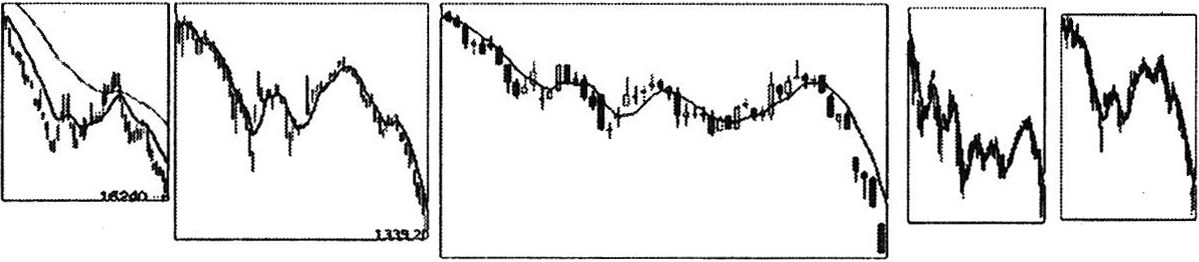
\includegraphics[width=0.88\linewidth]{images/5-1假双底.jpg}
\caption{假双底}\label{fig:false-double-bottom}
\end{figure}

\textbf{假双顶}

如图\ref{fig:false-double-top}。

\begin{figure}[htbp]
\centering
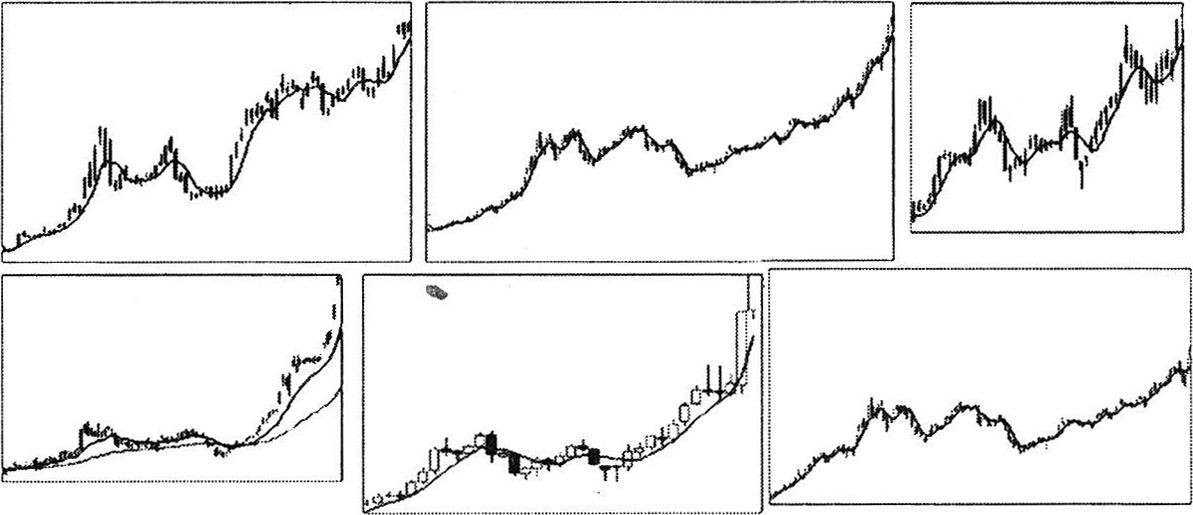
\includegraphics[width=0.8\linewidth]{images/5-2假双顶.jpg}
\caption{假双顶}\label{fig:false-double-top}
\end{figure}

\textbf{跨过顶部是天空}

\begin{figure}[htbp]
\centering
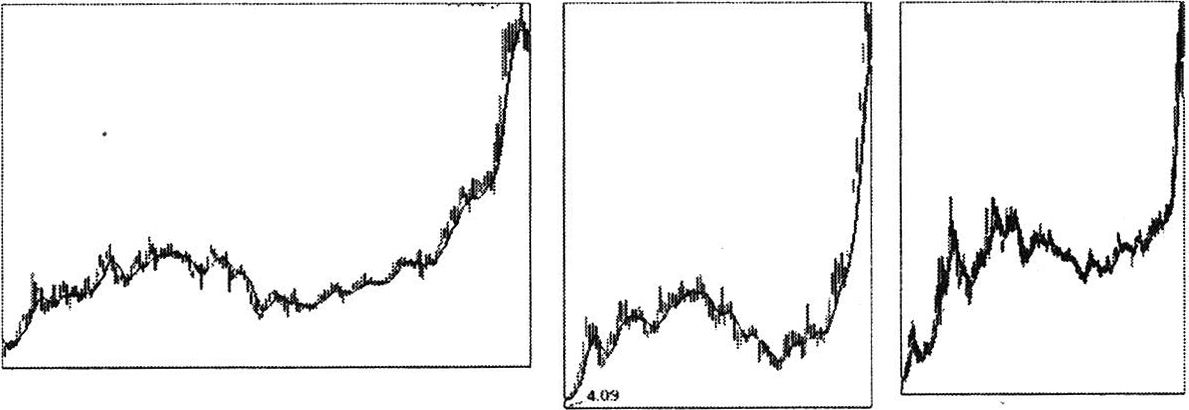
\includegraphics[width=0.88\linewidth]{images/5-3跨过顶部是天空示例图.jpg}
\caption{跨过顶部是天空}\label{fig:sky-beyond-top-example}
\end{figure}

我们不难发现，“跨过顶部是天空”的未来走势，通常都是比较壮观的。它用更长时间的横向整理，换取了未来更大的波动幅度。而假双底其后的下跌通常都是非常迅速的，但很多时候是熊市中的最后一跌，而在创出新低不远处最终见底。假双顶也是在市场中经常出现的一种形态，其后也会经历进一步上涨。由于假双底和假双顶都是波浪理论中“ABC调整”中的一小部分，确切地说应该只属于之字形调整。而“ABC调整”还有可能是平坦形［C浪不创A浪的低（高）点］。甚至在平坦形调整中还会出现更为强劲（疲弱）的奔走形［B浪创出新高（低）］。也就是说，市场的ABC三浪调整形态有一部分不属于假双底（顶），而这种形态的后期走势更具趋势特征。

\textbf{平坦形调整}

\begin{figure}[htbp]
\centering
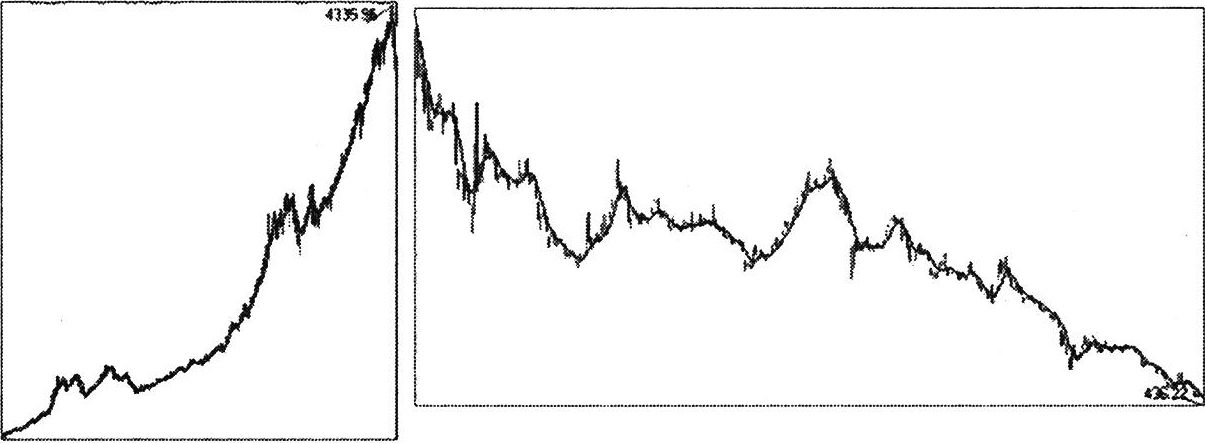
\includegraphics[width=0.88\linewidth]{images/5-4平坦形调整示例图.jpg}
\caption{平坦形调整}\label{fig:flat-adjustment-example}
\end{figure}

其实，按照这种从经典理论的误区中演化出来的反向交易策略，还可以包括“反缺口理论”。如果赌“逢缺口必回补”的交易者被扫地出门只是早晚的事情，那么我们就可以找到一种能够获利的策略。我们可以每逢向上缺口出现就买入，并且在缺口下方0.5倍缺口幅度的位置设置止损点。如果缺口不回补，我们就“永远”持有。这是一种失败率较高的方法，至少很大比例的交易我们是无法获利的。但如果真的买到了上证指数1996年初630点那样的缺口，那将是一笔可以让你获利极其丰厚的交易。在我看来，最好的交易策略是那种靠偶然事件改变命运的交易策略。这种方法虽然理论上可行，但是我绝对没有建议大家使用的意思，我相信有更好的获利策略。当然，这里只是介绍一种思路，\textbf{通过大众的误区来实现获利}。知识就是力量，而别人的无知同样是你的力量。从某种意义上来讲，我们不但可以从人性的偏向中寻找获利的策略。与此类似的，我们仍旧可以从经典理论的误区中寻找获利的策略。先不说所谓的理论正确与否，单单是大多数人都相信这一点，在市场面前就是不小的问题。海龟交易法则在被大众认可与仿效学习后，效果不是大打折扣了吗？要知道这可是与人性相逆的策略。如果是顺应人性的理论，那么一定会产生能够获利的“反理论”。

\subsection{择强汰弱}

{\kaishu
熊市不做头，牛市不做底。

\hfill ——金融帝国

各股形态形成的市场环境，往往比形态本身更为重要。

\hfill ——金融帝国
}

1999年5·19行情前夕，我的一个同学建议我买入西安民生。我打开走势图一看，怎么能买这样的股票呢？该股从4元涨至7元，在形成头肩顶后破位下跌。那时的价位好像是5.3元，并且一周后见到4.99元。我正在为没有买入而庆幸，但该股一个多月后涨至13.5元，并且连续拉出了7个涨停板！

\begin{figure}[htbp]
\centering
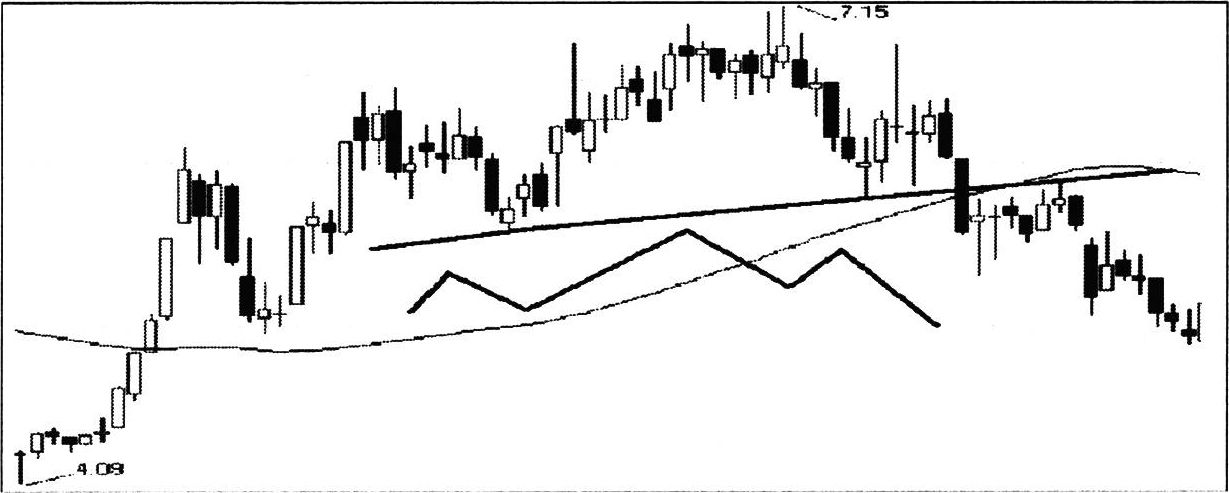
\includegraphics[width=0.88\linewidth]{images/5-5西安民生股价走势.jpg}
\caption{西安民生股价走势}\label{fig:xian-minsheng-chart}
\end{figure}

2000年底我在选股时为了最大程度地规避风险，而买入一只长期筑底的股票600788达尔曼。当时的理由很简单，第一，业绩优良、净资产高、未分配利润高；第二，1999年之前下跌50％以上，并且之后又横向整理了将近两年；第三，长期形态走出了标准的底部大三角形，并且向上突破上边线。当时我已经不会再“空手接飞刀”似的买入正在下跌的股票，但还存在占市场便宜的愚蠢念头。结果该股在未来一年多的时间内从15元跌至0.2元！

我不否认上述两个案例最终的结果很大程度上受到大盘的影响，但是谁也不能否认它们比大盘更强和更弱。这其中到底存在什么样的奥秘呢？当然，这其中有下一节会介绍的顶部与底部的误区。但一个更为重要的因素是，我在强弱上是逆势的！

何谓顶部？上涨之后出现的转折点。请注意，顶部形成的前提是之前必定为上涨行情。那么在熊市中能够上涨的股票，只能说明它比大盘强！而自由落体式下跌的股票是无所谓做顶的！那么能够做顶的股票，必定是熊市中的强势股。强通常有强的道理，并且强于大盘的股票，通常会继续强于大盘。这就是熊市不做顶的原因，而牛市不做底的道理也是相同的。如此一来，只能够说明，我买入的股票都是避强留弱的，那么经常跑输大盘就不足为奇了。原来，我输就输在了弃强留弱的误区上。

在我吸取了这种经验教训后，我得出了一种截然相反的选股策略。作为市场上弱势群体的我，不可能知晓个股基本面的真相，那么选股就必须用纯技术派的方式来解决。什么样的股票是好股票呢？答案很简单，比大盘强的股票就是好股票！而且越比大盘强的股票就越好。对于技术分析而言，从上千只股票中选股是一件很困难的事情，但这样一来，这个难题就彻底解决了。我经常发现，市场中一个臭不可闻的垃圾股在不断上涨，我越是不知道它为什么涨，它就越是涨个不停，而当我知道它上涨的原因以后，它就开始下跌了！

当然，这种方法的前提是，后期必须有大势的配合，因为个股也难抵大势。并且买入强势股的思路，是“不求价、只求势”的，必须有绝对的止损点作为配套。离开了这两个前提，这种方法的风险就极大了。但是，只要能够有绝对的止损点，什么样的股票对于你来说风险都是一样的！

\subsection{抛弃底部选股策略}

{\kaishu
买入第二年的股票。

\hfill ——一位老股民对我的忠告

抄底思路运用在大盘上是可以的，但运用在个股上就绝对是一个骗局！

\hfill ——金融帝国
}

曾经有一位老股民指点我“买入第二年的股票”，所谓第二年的股票就是去年上涨过一波的股票。当时我对这种买高不买低的思维方式嗤之以鼻，而倔强地坚持自己的“底部策略”。多年之后，我才感悟到前辈此话的真谛。

我进入股票市场看的第一本书是青木的《战胜庄家》，并且对该书的作者极为崇拜。此后我又寻找并且购买了他所有的著作，所以可以说他是我炒股理念最早的启蒙老师。青木推崇的观念非常不错，他指出止损点的重要性；顺势而为的重要性；不要因为价格高而卖出股票……他为了形象地说明，将股票分为四个阶段：底部阶段、上涨阶段、顶部阶段、下跌阶段。并且反复指出，永远不要持有第四阶段的股票。

青木对我的启发是巨大的，甚至可以算是我没有见过面的恩师！但就是这张“股价阶段循环图”将我引入一种思维误区。青木的观点是，在上涨中途买入股票是可以的，但最好是在底部阶段结束后，放量突破时建仓。这给了我一种错觉，认为股价的波动是循环的。并且被我贪低的本能所利用！

那时开始，我就误认为好股票都是经过长期下跌，并且长时间在底部整理，最终放量突破的。我不会买入正在下跌的股票，而是寻找大幅下跌后长时间横盘筑底的股票，并且等待突破而买入。我的下意识里认为，股票的涨跌是循环的，底部阶段过后就能涨回到原来的高点。也许青木本人和我都是本能地希望既求势又不丢价吧。

事实上，对于大盘而言，下跌能够成为未来上涨的理由，所以指数没有不可逾越的顶部。但股票不同！股票的基本面是可以变化的，即使基本面不变化，那么强弱的循环可能也需要十年的时间。而在这（十年的一半）五年中，一类股票会反复走强，而另一类的股票会反复走弱。1997年是绩优股的天下，而2007年同样是绩优股的天下。虽然深万科还能够继续重演十年前的辉煌，但曾经的四川长虹早已今非昔比，更不用说已经离开我们的达尔曼了。所以即使概念循环一遍，也不等于同样的股票也会循环。大盘是能够不断循环的，毕竟股民的人性是很难改变的。但对于个股而言，它更像是人的一生，是在经历一个不可逆转的轨迹，生老病死后就会离开我们的市场。即使股票真的有重生，那也需要一个漫长又漫长的过程，并且这也不是什么必然的现象。事实上，抄底思路运用在大盘上是可以的，但运用在个股上就绝对是一个骗局！

如果我跳不出“高低”的思维束缚，那么我就注定在趋势之路上一事无成。最终的结论是：除非我的持股周期超过五年，否则更多考虑价格的高低是没有任何意义的！只要我顺势、只要我使用绝对的止损点，那么再考虑其他的问题都是多余的！如果好股票从低点涨到高点需要5年的时间，即使我做足了第一年，那么后4年我干什么去呢？我又该如何应对4年间不断出现的从半空中起步的牛股呢？

1999年5·19行情时，我买入的是000625长安汽车。从复权走势图来看，该股1997年6月上市，价位为9.71元。其后一路下跌，并在1998年8月见底于3.58元。在此后的9个月内，该股一直横向整理，并且在5·19行情走出突破。当时，它极其符合我的选股条件，因此重仓买入。整个5·19行情，该股也不过涨到5.47元，明显弱于大盘。此后该股又回调至3.81元，在2000年的行情中，该股涨至9.21元；而在2003年的大熊市中，不可思议地涨至19.79元！

通过对历史上长线大牛股的统计发现，距离最低点越远发动的行情通常越壮观。或者说，长线大牛股都是越来越强劲地上涨，当达到最为强劲的极端时，就是形成长期顶部的时刻了。无论是1997年的长虹、发展、湖北兴化，还是2000年的亿安科技、海虹控股、青鸟天桥，都在反复证明这一点！

这说明，如果说一个长期概念能够持续走牛5年之久的话，那么我们买入的点位越接近顶部、越远离底部，我们的获利速度就越快！往往顶部都是突然从极强转变为极弱，不需要像底部那样有长时间的过渡期。

当然这是通过对历史上最为强劲的大牛股进行统计而得出的结论。对于一般的长期牛股而言，有可能最后的五浪并非将强劲演化为极致。但无论如何，三浪上扬，或者说是主升浪都是非常强劲的！

这好像又回到了波浪理论。按照波浪理论的说法，一浪只不过是长期上涨的预演罢了，甚至还会被其后的二浪大幅度地吞没，所以一浪是最弱的；三浪作为主升浪，从概率上来看是多数股票最为强劲的一波上涨；而五浪是收尾浪，部分股票能够走出“延长五浪”，将强劲发挥到极致。对于超级大牛股而言，最强的疯涨不是来自于三浪，而是来自于五浪；但对于大部分的股票而言，三浪强于五浪的概率更大一些；但无论如何，一浪都会是最弱的！

那位前辈所谓“买入第二年的股票”的观点，同波浪理论不谋而合。他并不精通波浪理论，但其极高的悟性让我深感佩服！在我看来，波浪理论的精髓不在于精确数浪，而在于波浪理论中最为宝贵的思想。这样一来，我的选股策略就从“底部突破”转变为“跨过顶部”。我通常买入随中期牛市上涨过一波，而在其后的中期熊市中能够拒绝调整的股票。或者是虽然经历过小幅下跌，但在中期熊市的底部时已经创出新高的股票。对于我来说，中期熊市的意义完全不是给我低价买入股票的机会，而是能够帮我将好的股票过滤出来。我曾经将其戏称为“水落石出”。

现在回想曾经的底部策略，不过是一种选择弱势股的策略。这就注定了我由于贪低的误区，而使得我曾经的持股成为弱势股的集中营。在我看来，大多数股民的本能中，都存在着选择弱势股的天赋！

\subsection{万绿丛中一点红}

什么是最为常见的底部形态呢？曾经我认为，双底是最为常见的底部形态，或者底部是盘整出来的。慢慢地，我发现对于大盘而言，很难找到标准的双底形态，基本上都是“砸”出来的底部；而对于个股而言，长时间盘整的底部并不难找到，但是它们其后的上涨通常并非很强。而真正的强势股，都是宽幅震荡后走出突破的股票。

一只从10元跌至5元，并且在5元至6元间长期整理筑底的股票并非好的股票，即使底部真的成立，那么未来的上涨也并非壮观。而如果一只从10元至5元来回大幅震荡的股票，那么突破10元后将会有大幅度的上涨。主升浪涨得最多的股票，通常是二浪大幅震荡的股票，震荡幅度越大越好；而五浪涨得最多的股票，通常是四浪运行得非常紧凑的股票，越简单、越紧密（走成一条线）就越好。至于大幅下跌后，走出双底图形的股票，基本上都是靠不住的。

对于大盘而言，很难走出什么长期盘底的走势，这一点是由“股市层次理论”所决定的。有意思的是，双底在大盘的历史底部也很难找到。真正常见的底部，通常都是失败双底（或者三重底）后快速砸出来的。通常而言，大盘会沿着一个下降通道下跌。其后会尝试横向整理筑底，这种横向整理会盘出下降通道上轨。这种尝试做底的横向整理基本上都会失败，而其后会快速下跌创出新低。这个新低就是最终的底部，而且停止于前期盘出下降通道的上轨处。简单地说就是，盘出下降通道后，再“踩一下”上轨就是底部。

\begin{figure}[htbp]
\centering
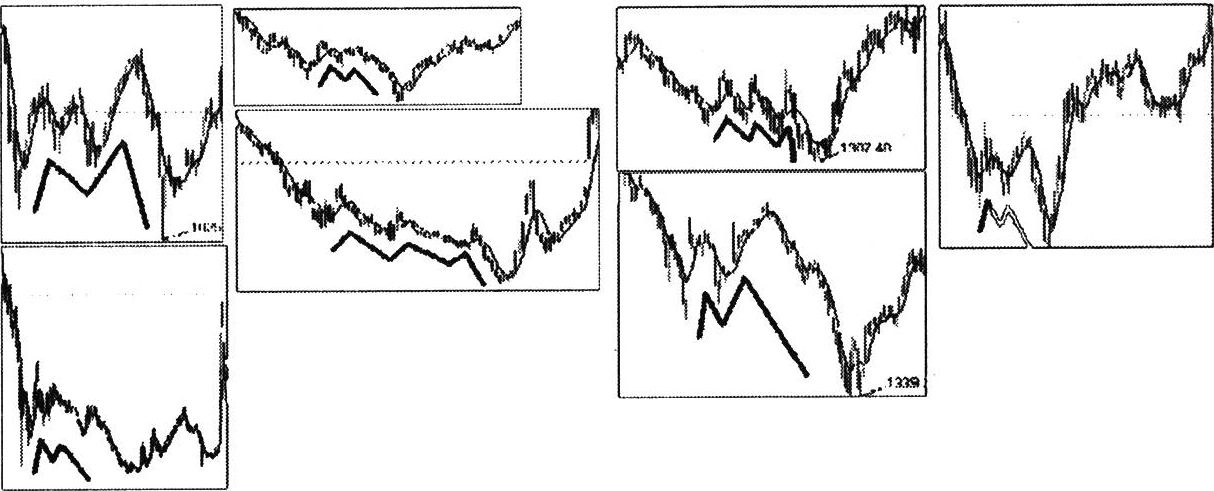
\includegraphics[width=0.88\linewidth]{images/5-6万绿丛中一点红示例图.jpg}
\caption{万绿丛中一点红示例图}\label{fig:one-red-among-green}
\end{figure}

大盘的底部通常是“砸”出来的，而个股的底部（事后才能看出）通常是震荡出来的。那么大盘在恐慌性的最后一跌中，我们该如何选股呢？答案很简单，就是“万绿丛中一点红”。能够在底部快速下跌的恐慌中收出红盘的股票，就是好的股票。道理同样简单，我们不知道哪只股票好，但恐怖的大盘就是最好的“试金石”！

\subsection{行情扩大器}

{\kaishu
无论牛市还是熊市，通常都是80％的股票弱于大盘，而20％的股票大大强于大盘。而这20％大大强于大盘的股票，正是你不敢买入的股票。

\hfill ——金融帝国
}

我的炒股方法基本上是以大盘为背景的，中期牛市持股、中期熊市持币。我不知道市场中是否有在中期熊市也能必然获利的高手。常理说，一轮牛熊循环下来，七赔、两平、一赚。那么能够在中期熊市中获利的人，肯定连1％都不到！我自叹不是那不足1％的高手，所以熊市中我会休息。当然这不包括，我在中期熊市末端，对逆势股票提前建仓的操作。

对于大多数股民而言，股市绝对不是一个“时间就是金钱”的场所。牛市比熊市更容易获利是无可厚非的。如果你连在牛熊循环中获取巨大的财富都做不到，那么还是学会在熊市中休息吧。大多数股民的问题不在于能否区分中期的牛熊市；而是他们总是自信地不愿意区分。

事实远远没有这么简单，“中期牛市持股；中期熊市持币；特定幅度的整理市道亏损”才是趋势跟踪者的全部。如果你能够甘心付出试错成本，那么判断市场并不复杂。但如何选股是一个很重要的问题。无论牛市还是熊市，通常都是80％的股票弱于大盘，而20％的股票大大强于大盘。如果你从来没有感受过大赚指数而没有赚到什么钱，那么你绝对不是一个真正的股民。要知道，大大强于大盘的股票，无论是在信念上、还是在本能上，都是股民不敢买入的股票！甚至在你没有意识到大盘的底部已经形成的时候，好的股票早已经大步向前飙升起来了。

对于新股民而言，前面的技巧你可能无法运用得得心应手，甚至你的本能都无法支持你做到。那么我告诉你一个更简单的办法：新股和除权是行情的扩大器。在大盘底部上市的新股、以及除权的股票，未来的涨幅通常会大于大盘；而在大盘顶部上市的新股、以及除权的股票，未来的跌幅通常会大于大盘。这个命题同样是基于概率产生的，而无法保证结果一定会怎么样。但以我多年的观察来看，效果确实不错。如果这个你还做不到，那就只好买入指数基金了。股民对于选股这个问题上，存在太多的误区。其实买入指数基金就能够保证你的收益与大盘同步，这要好于大部分交易者的实际战绩。交易是一门“舍”的艺术，当你舍去了暴利的黑马，那么你也规避了弱于大盘的风险。

\clearpage
